

\begin{table*}[ht]
\caption{
    Main experimental results on GAIA and SimpleQA benchmarks. \method is built upon Smolagents framework. All the results are using the pass@1 metric. The best results are shown in \textbf{bold}.
  }
  \label{tab:main}
  \centering
  \resizebox{0.95\textwidth}{!}{
      \begin{tabular}{llcccccccc}
        \toprule
          \multirow{2}{*}{\makecell[l]{\textbf{Agent} \\ \textbf{Framework}}} & \multirow{2}{*}{\makecell[l]{\textbf{Reflective} \\ \textbf{Method}}} & \multicolumn{4}{c}{\textbf{GAIA (\%)}} & \multicolumn{4}{c}{\textbf{SimpleQA (\%)}} \\
        \cmidrule(lr){3-6}  \cmidrule(lr){7-10}
       & & Level 1 ($\uparrow$) & Level 2 ($\uparrow$) & Level 3 ($\uparrow$) & Total ($\uparrow$) & Corr. ($\uparrow$) & Incor. ($\downarrow$) & N.A. ($\downarrow$) & C./Att. ($\uparrow$) \\
        \midrule
        \rowcolor{gray!15}
        \multicolumn{10}{c}{\textit{Backbone LLM: GPT-4.1}} \\
        % \midrule
        ReAct & - & 41.51 & 33.72 & 7.69 & 32.12 & 61 & 19 & 20 & 76.25 \\
        ReAct & Reflexion & 49.06 & 34.88 & 15.38 & 36.36 & 71 & 21 & 8 & 77.17 \\
        ReAct & Self-Refine & 39.62 & 39.53 & 11.54 & 35.15 & 74 & 18 & 8 & 80.43 \\
        Smolagents & - & 56.60 & 47.67 & 19.23 & 46.06 & 72 & 16 & 12 & 81.82 \\
        Smolagents & Reflexion & 56.60 & 54.65 & 19.23 & 49.70 & 79 & 20 & \textbf{1} & 79.80 \\
        Smolagents & Self-Refine & 58.49 & 52.33 & 23.08 & 49.70 & 78 & 18 & 4 & 81.25 \\
        {Smolagents} & \textbf{\method (ours)} & \textbf{71.70} & \textbf{55.81} & \textbf{38.46} & \textbf{58.18} & \textbf{83} & 15 & 2 & \textbf{84.69} \\
        \midrule
        \rowcolor{gray!15}
        \multicolumn{10}{c}{\textit{Backbone LLM: Gemini-2.5-pro}} \\
        % \midrule
        ReAct & - & 56.60 & 45.35 & 30.77 & 46.67 & 55 & 16 & 29 & 77.46 \\
        ReAct & Reflexion & 56.60 & 47.67 & 30.77 & 47.88 & 70 & 18 & 12 & 79.55 \\
        ReAct & Self-Refine & 56.60 & 44.19 & 34.62 & 46.67 & 62 & 24 & 14 & 72.09 \\
        Smolagents & - & 54.72 & 52.32 & 34.62 & 50.30 & 76 & 18 & 6 & 80.85 \\
        Smolagents & Reflexion & 60.38 & 52.33 & \textbf{38.46} & 52.73 & 78 & 22 & \textbf{0} & 78.00 \\
        Smolagents & Self-Refine & 60.38 & 50.00 & 34.62 & 50.91 & \textbf{81} & 17 & 2 & 82.65  \\
        {Smolagents} & \textbf{\method (ours)} & \textbf{67.92} & \textbf{60.47} & \textbf{38.46} & \textbf{59.39} & \textbf{81} & \textbf{13} & 6 & \textbf{86.17}  \\
        \bottomrule
      \end{tabular}
     }
\end{table*}


\subsection{Experiment Settings}


\noindent\textbf{Datasets.} To evaluate the general task completion performance of \method, we conduct comprehensive experiments on the following datasets with complete agentic settings. 
\begin{enumerate*}[label=\arabic*)]
    \item \textbf{GAIA} \citep{mialon2023gaia} is a general AI assistant benchmark that evaluates AI agent's ability to complete real-world tasks, covering multi-step reasoning, fact checking, web browsing, and tool usage. We select the validation set.
    \item \textbf{SimpleQA} \citep{wei2024measuring} is a challenging benchmark that evaluates the ability to answer fact-seeking questions. Due to resource limitations, we randomly select 100 samples from the test set.
\end{enumerate*} 
Note that for constructing the planning errors, we leverage \textbf{HotpotQA} \citep{yang2018hotpotqa} and \textbf{MuSiQue} \citep{trivedi2022musique} datasets, ensuring no overlap with the test benchmarks while challenging the agent's diverse capabilities.

\noindent\textbf{Baselines.} We compare with various baselines to validate the effectiveness of our proposed method. In particular, we select Reflexion \citep{shinn2023reflexion} and Self-Refine \citep{madaan2023self}, which are standard retrospective reflection methods. We omit \citet{wang2024devil} as it targets step-level anticipation and is not directly applicable to GAIA-style long-horizon planning tasks. Also, we compare with several agent frameworks, such as ReAct \citep{yao2022react}, Smolagents and its Open Deep Research (ODR) system \citep{smolagents}, AutoAgent \citep{chen2023autoagents}, Magnetic-1 \citep{fourney2024magentic}, HAL \citep{hal}, OWL \citep{hu2025owl}, and OAgent \citep{zhu2025oagents}.



\noindent\textbf{Evaluation Metrics.} For GAIA, we use standard ``pass@1'' which refers to the percentage of problems solved correctly when 1 candidate solution is sampled per task. For SimpleQA, we follow the standard evaluation to report \textbf{Correct} (\textbf{Corr.}), \textbf{Incorrect} (\textbf{Incor.}), \textbf{Not Attempted} (\textbf{N.A.}), and \textbf{Correct Given Attempted} (\textbf{C./Att.}), which refer to the number of correct, incorrect, not attempted, and correct given attempted answers out of all the answers, respectively.

\noindent\textbf{Agent Implementations.} \method (built upon Smolagents) operates under a maximum budget of 20 execution steps and is equipped with standard web search and webpage navigation tools. To satisfy the multimodal tool requirements of GAIA tasks (e.g., involving images or audio), we additionally provide a set of lightweight modality-specific inspection tools. 
Importantly, all compared methods are evaluated under the same tool access and execution constraints to ensure a fair comparison in our main experiments. Further implementation details are deferred to Appendix~\ref{appendix:imp}.


\definecolor{box-blue}{HTML}{8E8BFE}
\definecolor{box-red}{HTML}{FEA3A2}
\definecolor{box-gray}{HTML}{F2F2F2}
\definecolor{error-tag}{HTML}{D32F2F}

\begin{figure*}[ht]
\centering
\begin{tcolorbox}[colback=white, colframe=gray!50, arc=2mm, boxrule=0.5pt, title=\textbf{Qualitative Analysis: An Example From GAIA Level 3 Task}]
    \begin{minipage}[t]{0.45\textwidth}
        \small \textbf{\faSearch \ Task:} \\
        \small Eva Draconis has a personal website which can be accessed on her YouTube page. What is the meaning of the only symbol seen in the top banner that has a curved line that isn't a circle or a portion of a circle? Answer without punctuation.
    \end{minipage}
    \hfill
    \vrule \hfill 
    \begin{minipage}[t]{0.48\textwidth}
        \small \textbf{\faMapSigns \ Ground Truth Trajectory:} \\
        \footnotesize
        \begin{enumerate*}[label=\arabic*., itemjoin={\ $\rightarrow$\ }] 
            \item Google Eva Draconis YouTube \item Find her website URL in her about section \item Enter to identify symbols and their meanings \item Find the only symbol that matches all the requirements \item Note the meaning ``War is not here, this is a land of peace.''
        \end{enumerate*}
    \end{minipage}
    \small
    \begin{tcolorbox}[colback=box-gray, colframe=gray!40, arc=1mm, boxrule=0.5pt, title=\textbf{\faHistory \ Step 1--14: Plans, Actions, and Failure}]
        Agent initiated a multi-step search strategy: scraping YouTube ``About'' sections, scanning social media (Facebook/Patreon), and querying Google Images. \\
        \textbf{Outcome:} All attempts resulted in 404/403 errors or irrelevant results (e.g., Space.com forums), as the primary site (\textit{orionmindproject.com}) was defunct.
    \end{tcolorbox}

    % \vspace{2mm}
    \begin{tcolorbox}[colback=box-blue!10, colframe=box-blue, arc=1mm, boxrule=1pt, title=\textbf{\faLightbulbO \ Dynamic Re-Planning (Step 15)}]
        \textbf{Thought:} All searches for \dots for orionmindproject.com and Eva Draconis site are futile \dots A new approach is mandatory. \\
        \textbf{Re-plan Proposal:} The agent proposed to double-down on Wayback Machine visual captures, attempting to retrieve and process the banner image via the \texttt{inspector} tool.
    \end{tcolorbox}

    % \vspace{2mm}
    \begin{tcolorbox}[colback=box-red!10, colframe=box-red, arc=1mm, boxrule=1pt, title=\textbf{\faCheckSquareO \ Plan Reflection \& Revision}]
        \textbf{Reflection Analysis:} \textcolor{error-tag}{\textbf{[ineffective\_tool\_selection]}} \\
        The plan \dots to locate and process a banner image \dots but \dots visit\_webpage tool cannot retrieve images, and the inspector tools require a publicly accessible image URL \dots The plan does not include a strategy to overcome this technical constraint. \\
        \textbf{Revised Plan:} \textbf{Pivot from visual retrieval to \textit{source-code} excavation.} Propose using `visit\_webpage' to extract the HTML or text contents of the homepage for archived homepage snapshots of \texttt {orionmindproject.com}.
    \end{tcolorbox}

    % \vspace{2mm}
    \textbf{\faRocket \ Final Execution (Step 16-18):} \\
    $\rightarrow$ \textbf{Action:} \texttt{visit\_webpage} on archived \textbf{source code.} \\
    $\rightarrow$ \textbf{Key Observation:} Detected a hidden textual anchor: \textit{``the alien writing on the top is... Kesovan symbols... see what they mean here.''} \\
    $\rightarrow$ \textbf{Result:} Accessed symbols glossary. Symbol 10 (\textit{Leaning curve}): \textbf{``War is not here this is a land of peace''} \checked
\end{tcolorbox}
% \vspace{-5pt}
\caption{An example of how \method triggers dynamic re-planning, reflects on the plan based on the planning errors, and finally revises the plan to avoid failure.}
% \vspace{-10pt}
\label{fig:qualitative_analysis}
\end{figure*}

\subsection{Main Results}
Table~\ref{tab:main} presents the primary experimental results comparing \method  against various baselines on the GAIA and SimpleQA benchmarks. To ensure a rigorous and equitable comparison, we maintain strictly identical settings, such as tool set and inference parameters, across all evaluated methods, thereby eliminating confounding factors related to environmental configuration.



\noindent\textbf{Quantitative Analysis.} Table~\ref{tab:main} presents the performance of \method compared to representative agentic and reflective baselines on GAIA and SimpleQA benchmarks. On GAIA, \method achieves the highest total score of $58.18\%$ (GPT-4.1) and $59.39\%$ (Gemini-2.5-pro), representing an average improvement of $17.14\%$ and $11.68\%$ over baselines. Besides, the performance gap on Level 3 tasks, where \method outperforms baselines by $14.29\%$ on average, suggests that prospective reflection excels at high-complexity reasoning where error propagation is most severe.

On the SimpleQA benchmark, \method significantly enhances factuality, achieving an average improvement of $12.79\%$ in the Correct metric compared to all baselines across both LLM backbones. The simultaneous increase in the Correct Given Attempted metric ($6.08\%$ on average for GPT-4.1 and $7.73\%$ on average for Gemini-2.5-pro) and decrease in the Not Attempted metric ($12.29\%$ on average for GPT-4.1 and $4.00\%$ on average for Gemini-2.5-pro) indicate that our method allows agents to locate grounded information. Different from traditional methods to improve the factuality of an LLM without tools \citep{wang2025truthflow, cao2024personalized}, the performance gain under the agentic setting demonstrates that our proposed method results in a more comprehensive and robust system that further avoids hallucinations.




\noindent\textbf{Qualitative Analysis.} Figure~\ref{fig:qualitative_analysis} illustrates how \method handles a complex Level-3 GAIA task to \textit{identify the meaning of a specific symbol on Eva Draconis' personal website which can be accessed on her YouTube page}. The task is particularly challenging because both the target YouTube channel and the personal webpage 
% (\href{http://orionmindproject.com/}{orionmindproject.com}) 
is no longer active. While the agent initially struggles for 14 steps with empty pages and missing links, \method triggers a ``turning point'' at step 15 via prospective reflection. Recognizing that standard searches are futile, the agent performs dynamic re-planning to pivot toward the Wayback Machine. Crucially, to mitigate potential \textit{ineffective tool selection} problem, the revised plan shifts from direct image retrieval to source-code excavation. By extracting raw HTML via the ``visit\_webpage'' tool, the agent successfully locates the archived symbol description, completing a task that would otherwise result in a failure state.


\subsection{Comparison with Complex Agent Frameworks}
Beyond the controlled reflection-based comparisons in Table~\ref{tab:main}, Table~\ref{tab:comp_frame} situates \method within a broader landscape of sophisticated agent frameworks. These systems are typically evaluated under non-standardized and substantially more resource-rich settings, often involving more powerful tool access, different backbone models, larger action budgets, and specialized prompt or memory designs.
As a result, their reported performance is not directly comparable to our controlled experimental setting. We therefore cite these results directly from the original publications and present them separately to provide qualitative context rather than a strict head-to-head evaluation. Detailed configurations and sources for these agent frameworks are provided in Appendix~\ref{appendix:source}.


\begin{table}[ht]
\vspace{-5pt}
\caption{Comparative results on the GAIA validation set between various agentic frameworks. Results are directly cited from their respective original reports or other sources.}
\label{tab:comp_frame}
\centering
\resizebox{0.95\linewidth}{!}{
    \begin{tabular}{llcccc}
        \toprule
        \multirow{2}{*}{\textbf{Frameworks}}& \multirow{2}{*}{\textbf{Backbone LLM}} & \multicolumn{4}{c}{\textbf{GAIA (\%)}} \\
        \cmidrule(lr){3-6}
        & & L1 ($\uparrow$) & L2 ($\uparrow$) & L3 ($\uparrow$) & Total ($\uparrow$) \\
        \midrule
        \textbf{AutoAgent} & Claude-Sonnet-3.5 & 71.70 & 53.49 & 26.92 & 55.15 \\
        \textbf{Magnetic-1} & o1 & 56.60 & 46.51 & 23.08 & 46.06 \\
        \textbf{HAL Agent} & GPT-4.1 & 52.83 & 55.81 & 23.08 & 49.70 \\
        \textbf{HF-ODR} & GPT-4.1 & 58.49 & 50.00 & 34.62 & 50.30 \\
        \textbf{HF-ODR} & o1 & 67.92 & 53.49 & 34.62 & 55.15 \\
        \textbf{OWL} & GPT-4.1 & 71.70 & 50.00 & 26.92 & 53.33 \\
        \textbf{OAgent} & GPT-4.1 & 67.92 & 53.49 & 34.62 & 55.15 \\
        \midrule
        \textbf{\makecell[l]{Smolagents \\ + \method}} & GPT-4.1 & 71.70 & 55.81 & 38.46 & 58.18 \\
        \textbf{\makecell[l]{Smolagents \\ + \method}} & Gemini-2.5-pro & 67.92 & 60.47 & 38.46 & 59.39 \\
        \bottomrule
    \end{tabular}
}
\vspace{-10pt}
\end{table}

As shown in Table~\ref{tab:comp_frame}, \method outperforms significantly more complex multi-agent architectures (e.g., AutoAgent and OWL) by over $3\%$. These results underscore that effective prospective reflection can surpass simply increasing execution steps or orchestrating additional agent roles. Importantly, \method is \textbf{orthogonal} to these frameworks and can in principle be integrated as a reflection module to further improve their planning and execution robustness.


\subsection{Transferability}
Although we primarily instantiate \method within the Smolagents framework, we further evaluate its transferability across different agent architectures. Specifically, we integrate \method into a distinct agent framework, OWL~\citep{hu2025owl}. To ensure a fair comparison, we evaluate both variants under the same setting as in our main experiments (identical tool access, execution budgets, and hyperparameter settings), and report pass@1 accuracy on the GAIA validation set.



\begin{table}[ht]
% \vspace{-5pt}
    \caption{Transferability results across different agentic systems.}
    \label{tab:transfer}
    \centering
    \resizebox{0.85\linewidth}{!}{\begin{tabular}{lcccc}
        \toprule
        \textbf{Frameworks} & \textbf{Level 1} & \textbf{Level 2} & \textbf{Level 3} & \textbf{Total} \\
        \midrule
        \textbf{Smolagents} & 56.60 & 47.67 & 19.23 & 46.06 \\
         + \textbf{\method} & 71.70 & 55.81 & 38.46 & 58.18 \\
        \midrule
        \textbf{OWL} & 60.38 & 51.16 & 26.92 & 50.30 \\
         + \textbf{\method} & 73.58 & 58.14 & 42.31 & 60.61 \\
        \bottomrule
    \end{tabular}}
    \vspace{-5pt}
\end{table}



As shown in Table~\ref{tab:transfer}, \method consistently improves performance over the corresponding backbone, indicating that prospective reflection can serve as a general add-on module beyond a single agent implementation.


\subsection{Error Distribution}

To further reveal the error patterns exhibited by our proposed reflection mechanism, we analyze the reflective processes and error recognition of \method with GPT-4.1 backbone on the GAIA validation set. Across all 165 tasks, the defect rate, defined as the proportion of plans identified as risky among all updated plans, is $74.44\%$, revealing that most of the plans are reflected as carrying critical errors. As illustrated in Figure~\ref{fig:error_dist}, the error distribution is heavily skewed: insufficient constraint verification ($64.92\%$) and ineffective tool selection ($32.84\%$) account for nearly all identified errors.


This concentration suggests a fundamental gap in planning. While the agent aims for concise, high-level strategies, the high frequency of constraint-related and tool-related errors reveals that critical task boundaries and reasonable tool selection are often lost in abstraction. This indicates that for complex reasoning tasks, conciseness may come at the cost of operational rigor. Without explicit grounding in task-specific environments, the agent tends to neglect something that can be the key to completing the task correctly.

\begin{figure}[bh]
    \centering
    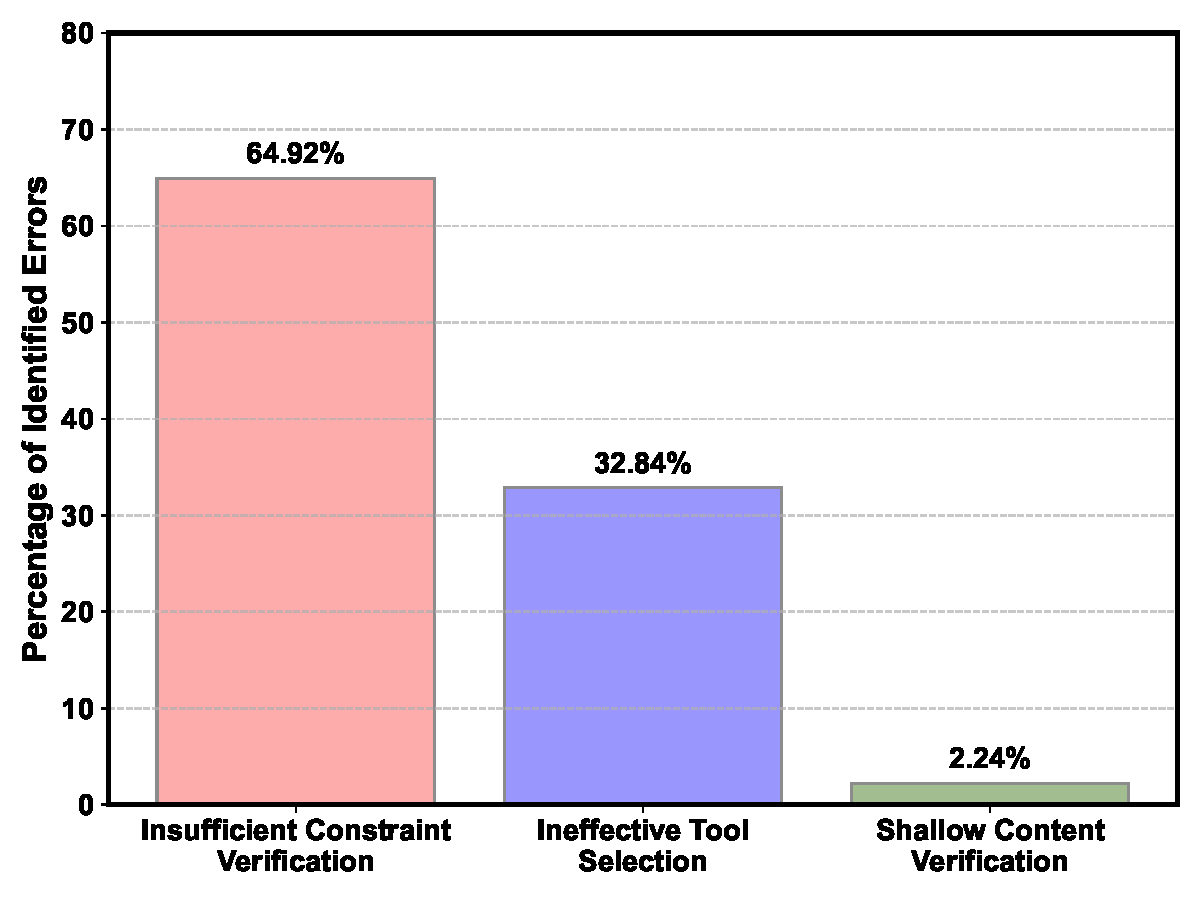
\includegraphics[width=0.85\linewidth]{img/error_dist.pdf}
    \caption{Error distribution of \method on GAIA using GPT-4.1 as the backbone LLM.}
    % \vspace{-10pt}
    \label{fig:error_dist}
\end{figure}

\subsection{Ablations}

To rigorously assess the individual contributions of the Planning Errors (PE) and Dynamic Re-Planning (DRP) modules, we conducted an ablation study using Smolagents as our baseline framework. The results, summarized in Table~\ref{tab:ablation}, isolate the impact of removing each component while keeping the experimental setting consistent.

\begin{table}[ht]
% \vspace{-5pt}
    \caption{Ablation studies on the planning errors (denoted as PE) and the dynamic re-planning (denoted as DRP). Results are from GPT-4.1 as the backbone LLM on the GAIA validation set.}
    \label{tab:ablation}
    \centering
    \resizebox{0.9\linewidth}{!}{\begin{tabular}{lcccc}
        \toprule
        \textbf{Method} & \textbf{Level 1} & \textbf{Level 2} & \textbf{Level 3} & \textbf{Total} \\
        \midrule
        Smolagents & 56.60 & 47.67 & 19.23 & 46.06 \\
        \method w/o PE & 58.49 & 53.49 & 23.08 & 50.30 \\
        \method w/o DRP & 54.72 & 54.65 & 34.62 & 51.52 \\
        \method & 71.70 & 55.81 & 38.46 & 58.18 \\
        \bottomrule
    \end{tabular}}
    % \vspace{-10pt}
\end{table}

\noindent\textbf{Planning Errors as Empirical Priors.} The ablated results indicate that the Planning Errors is essential for the transition from retrospective to prospective reflection. Removing it leads to a significant performance drop, particularly on Level 3 tasks (decreasing from $38.46\%$ to $23.08\%$). This aligns with our hypothesis that predicting future errors is inherently difficult without historical context. PE acts as an ``empirical prior'', grounding the prospective reflection and allowing the agent to anticipate and avoid potential pitfalls before execution begins.

\noindent\textbf{Dynamic Re-Planning as Compensation.} While PE aids in pre-execution error avoidance, the \textit{w/o DRP} variant reveals the necessity of runtime flexibility. Despite having access to historical error experiences, the agent may still fail to detect or mitigate every risk during the planning phase. The $6.66\%$ total performance gap between \method and \textit{w/o DRP} demonstrates that re-planning serves as a critical safety net, without which, the added complexity of prospective reflection might lead to rigid plans that the agent cannot recover from if a minor execution error occurs.


\subsection{Cost Analysis}
To evaluate the practical scalability of \method, we analyze its operational costs relative to performance on the GAIA validation set. We compare results of GPT-4.1 as the backbone LLM whose input price is \$2 per million tokens while the output price is \$8 per million tokens. As illustrated in Figure~\ref{fig:cost}, \method achieves a superior performance-cost trade-off compared to existing frameworks. While the baseline Smolagents costs \$46.31, our method reaches a highest score of 58.18\% with only a marginal 17.64\% cost increase (\$54.48). In stark contrast, advanced agents like HAL and HF-ODR incur significantly higher expenditures (\$74.19 and \$109.88, respectively) yet yield lower performance (49.70\% and 50.30\%).

\begin{figure}[ht]
    \centering
    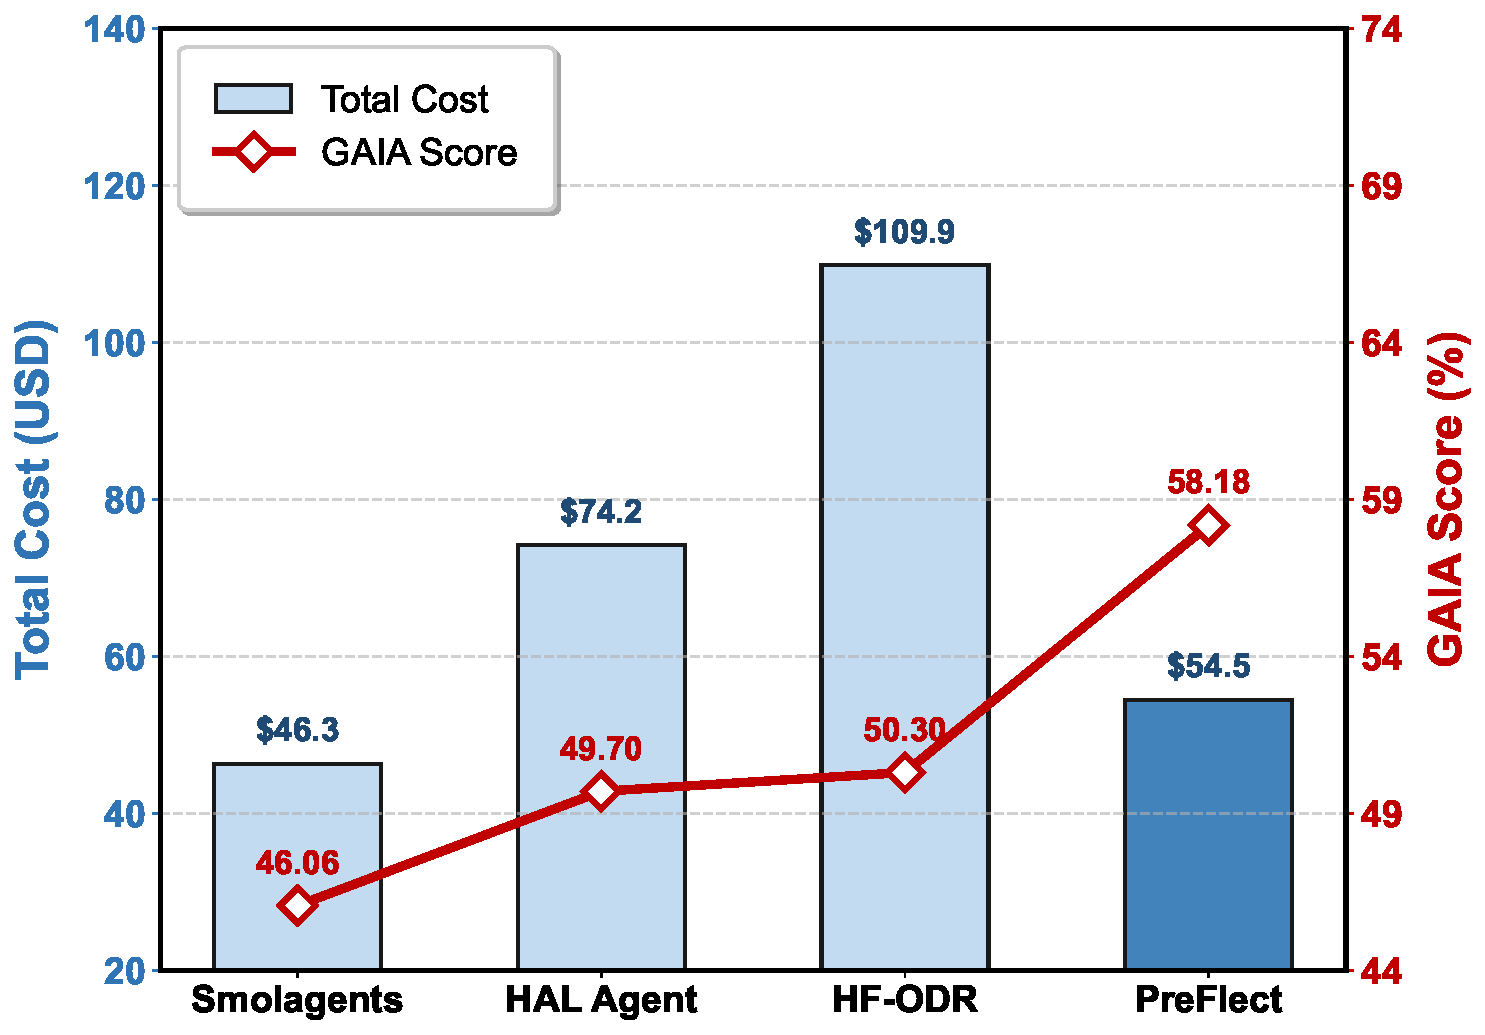
\includegraphics[width=0.95\linewidth]{img/cost_performance_v2.pdf}
    \caption{Performance-cost trade-off on the GAIA validation set. The primary axis shows the total cost (USD) and the secondary axis shows the corresponding GAIA scores.}
    \vspace{-10pt}
    \label{fig:cost}
\end{figure}


